\begin{figure}[t]
    \centering
    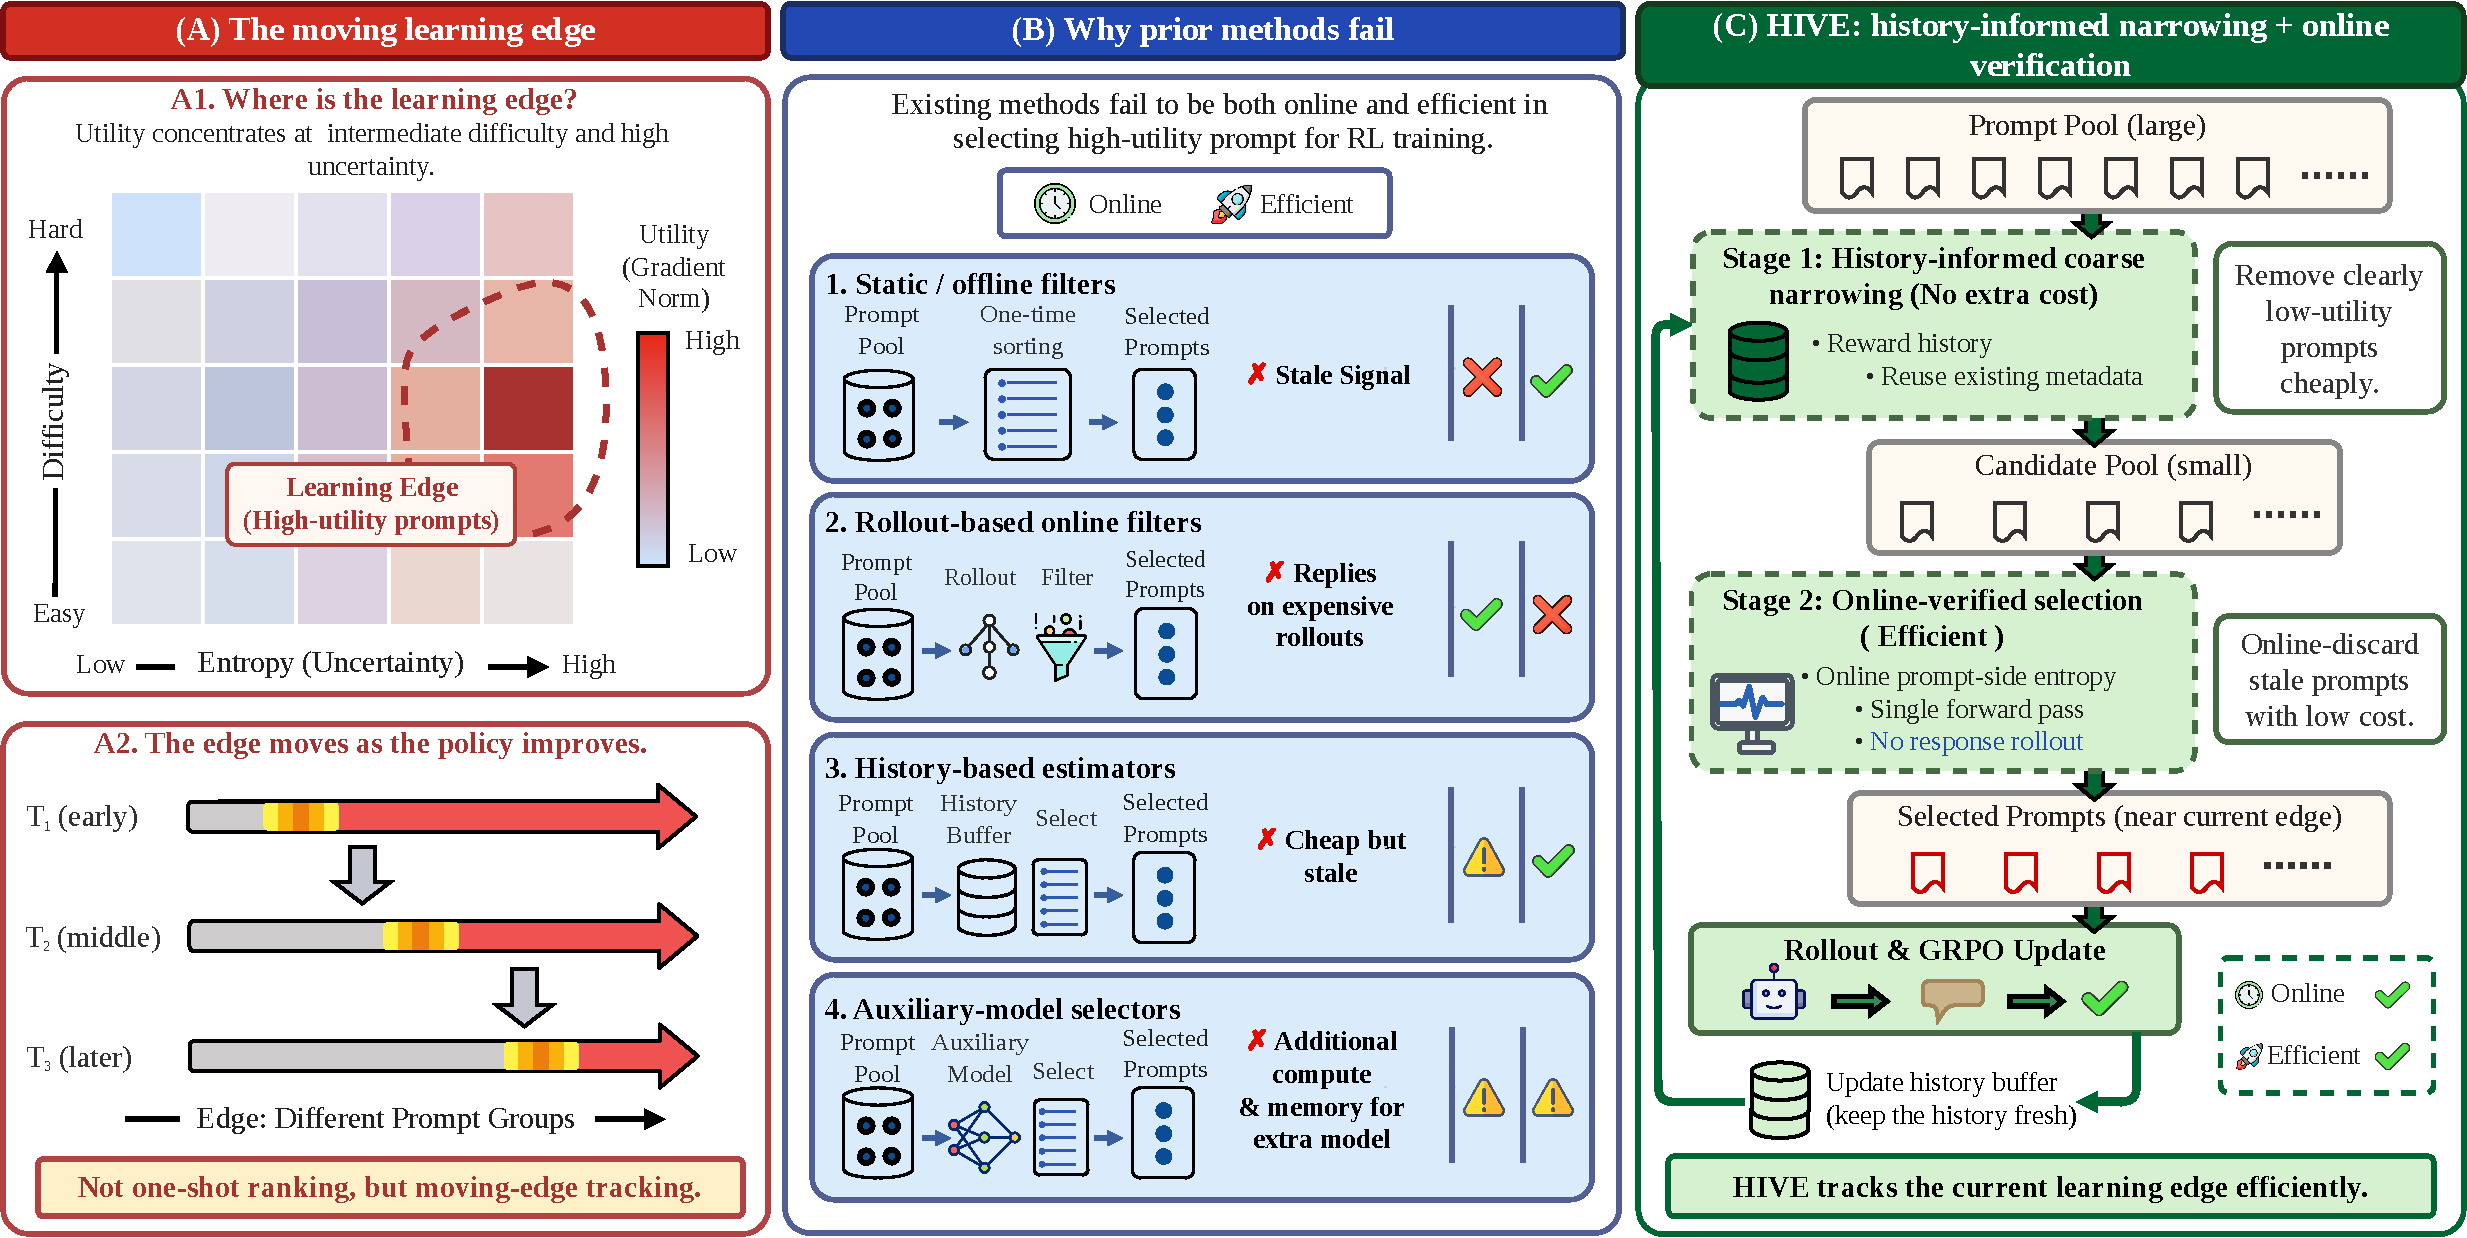
\includegraphics[width=0.98\linewidth]{figures/introduction/intro-fig-compare-motivate-1.pdf}
    \caption{\textbf{RLVR prompt selection is a moving-edge tracking problem.} (A) Utility concentrates at 
    intermediate difficulty and high uncertainty, and the learning edge is dynamic. 
    (B) Prior methods face limitations in efficiently selecting online high-utility prompts. (C) HIVE combines history-informed coarse narrowing with low-cost online 
    verification to track the current learning edge.}
    \label{fig:intro-compare-motivate}
    \vskip -0.2in
\end{figure}
% \red{1. re-write this caption 2.
%     delete precise. 3. redraw figure 3(d) to correspond to the A2 in figure 1. 4. shoud not be like curriculum, 
%     instead the utility of prompts across different step should be varying.}

\section{Introduction}
\label{sec:introduction}
Reinforcement Learning (RL) has emerged as a prevalent paradigm for fine-tuning large language models (LLMs), particularly for enhancing complex mathematical and logical reasoning capabilities~\cite{guo2025deepseek,yu2025dapo,tomihari2026learningdynamicsrlposttraining}. While advanced RL algorithms such as group relative policy optimization (GRPO)~\cite{shao2024deepseekmath} rely on rollout scaling to stabilize training and enhance model performance, they introduce a severe computational overhead~\cite{xu2025not,yu2025dapo,li2026stalefeedbackcoevolvingcritics}. In the training of those RL algorithms, a large portion of computational resources is wasted on generating rollouts for low-utility prompts that are either too trivial or too intractable for the current model. This results in vanishing gradients and wasted resources, providing no informative learning signal for model updates~\cite{zheng2025act,yu2025dapo,noukhovitch2025fasterICLR,verl2025}. Therefore, we investigate the following research question in this paper: \textit{how to identify prompts that are likely to produce useful gradients before rollout?}

Existing methods face limitations in efficiently selecting {high-utility} prompts in an online manner. Static or offline filters rank prompts before training using fixed heuristics, making them inexpensive but unable to adapt to the changing model during RL 
training~\cite{Wang2025ReinforcementLF,Li2025LIMRLI,ye2025limo}. Rollout-based online filters, such as dynamic sampling, better capture the current utility of each prompt by checking reward variance from newly generated responses~\cite{yu2025dapo,xu2025not,Chen2025LSPO,Ye2025PROF}. However, they already incur substantial rollout cost. History-based estimators such as GRESO~\cite{zheng2025act} avoid additional 
rollout cost by estimating prompt utility from past reward statistics, but those metadata becomes stale as the policy 
updates~\cite{zheng2025act,sun2025dots,li2026stalefeedbackcoevolvingcritics}. Auxiliary-model selectors, such as PCL~\cite{Gao2025PCL}, attach external or jointly trained predictors to estimate prompt difficulty or utility, introducing extra compute and memory during selection. 

% To understand what makes a prompt useful during RL training, we first conduct an empirical analysis of GRPO 
% training dynamics.  
% Among prompts with non-zero gradients, high response-side entropy prompts yield stronger learning progress at the same 
% rollout budget (Figure~\ref{fig:intro-a-b}b). More broadly, utility (\red{which we measured via length-normalized gradient norm}) concentrates at the intersection 
% of \red{intermediate difficulty} and high response-side entropy (Figure~\ref{fig:intro-a-b}c), which we term as 
% {learning edge}. However, the edge moves: prompts selected by those historical metadata quickly 
% lose real-time utility, whereas prompts verified under the current policy retain higher gradient norms 
% (Figure~\ref{fig:intro-a-b}a,\ref{fig:intro-a-b}d). Based on these observations, we conclude that an ideal prompt selection 
% framework for efficient LLM RL must be: \textbf{online} to track the moving learning edge, and \textbf{efficient} to avoid excessive overhead for selection.
% To identify what makes a prompt useful during RL training, we first empirically analyze GRPO training dynamics. Among prompts with non-zero gradients, those with high response-side entropy produce greater learning progress under the same rollout budget (Figure~\ref{fig:intro-a-b}b). More broadly, utility, measured by the length-normalized gradient norm, concentrates at the intersection of intermediate difficulty and high response-side entropy (Figure~\ref{fig:intro-a-b}c), which we refer to as the learning edge. However, this edge is dynamic: prompts selected using historical metadata quickly lose real-time utility, whereas prompts verified under the current policy retain higher gradient norms (Figure~\ref{fig:intro-a-b}a,\ref{fig:intro-a-b}d). These observations suggest that an effective prompt selection framework for efficient LLM RL should be \textbf{online}, to track the moving learning edge, and \textbf{efficient}, to avoid excessive selection overhead.
To identify what makes a prompt useful during RL training, we first empirically analyze GRPO training dynamics. Among prompts with non-zero gradients, those with high response-side entropy produce greater learning progress under the same rollout budget (Figure~\ref{fig:intro-high-entropy}). More broadly, utility, measured by the length-normalized gradient norm, concentrates at the intersection of intermediate difficulty and high response-side entropy (Figure~\ref{fig:intro-learning-edge}), which we refer to as the learning edge. However, this edge is dynamic: prompts selected using historical metadata quickly lose real-time utility, whereas prompts verified under the current policy retain higher gradient norms (Figures~\ref{fig:intro-history-staleness}); prompts move substantially among High, Low, and Zero utility classes across training steps (Figure~\ref{fig:intro-utility-shift}). These observations suggest that an effective prompt selection framework for efficient LLM RL should be \textbf{online}, to track the moving learning edge, and \textbf{efficient}, to avoid excessive selection overhead.
% To identify what makes a prompt useful during RL training, we first empirically analyze GRPO training dynamics. Among prompts with non-zero gradients, those with high response-side entropy produce greater learning progress under the same rollout budget (Figure~\ref{fig:intro-high-entropy}). More broadly, utility, measured by the length-normalized gradient norm, concentrates at the intersection of intermediate difficulty and high response-side entropy (Figure~\ref{fig:intro-learning-edge}), which we refer to as the learning edge. However, this edge is dynamic: prompts selected using historical metadata quickly lose real-time utility, whereas prompts verified under the current policy retain higher gradient norms (Figure~\ref{fig:intro-history-staleness}); prompts also move substantially among High, Low, and Zero utility classes across training steps (Figure~\ref{fig:intro-utility-shift}). These observations suggest that an effective prompt selection framework for efficient LLM RL should be \textbf{online}, to track the moving learning edge, and \textbf{efficient}, to avoid excessive selection overhead.


% To understand what makes a prompt useful for RL training, we first empirically examine GRPO training dynamics. Among prompts with non-zero gradients, those with higher response-side entropy yield greater learning progress under the same rollout budget (Figure~\ref{fig:intro-high-entropy}). More generally, utility, measured by the length-normalized gradient norm, is concentrated where intermediate difficulty and high response-side entropy intersect (Figure~\ref{fig:intro-learning-edge}); we refer to this region as the \emph{learning edge}. However, this edge shifts over time: prompts selected using historical metadata rapidly lose real-time utility, whereas prompts verified under the current policy maintain higher gradient norms (Figure~\ref{fig:intro-history-staleness}). Moreover, prompts frequently transition among High-, Low-, and Zero-utility classes throughout training (Figure~\ref{fig:intro-utility-shift}). These findings suggest that an effective prompt selection framework for efficient LLM RL should be both \textbf{online}, to track the moving learning edge, and \textbf{efficient}, to minimize selection overhead.

Based on previous analysis, we propose \textbf{HIVE} (\textbf{H}istory-\textbf{I}nformed \textbf{V}erification of the learning \textbf{E}dge), a dual-stage 
framework for rollout-efficient RLVR (Figure~\ref{fig:framework}). HIVE first performs history-informed coarse narrowing using 
reward trajectories and response-side entropies accumulated from previous training steps. This stage targets efficiency by retaining exploration probability for prompts that are around the edge. HIVE then utilizes prompt entropy as a high-fidelity and efficient proxy to perform online verification under the current policy, filtering stale candidates before the rollout phase.
% HIVE then performs online verification with prompt-side entropy 
% computed under the current policy. This stage restores online precision and filters 
% stale candidates before the rollout phase.

% Evaluation for HIVE is conducted across multiple reasoning benchmarks (e.g., {math, coding, and tool calling}) and models: Qwen3-4B~\cite{yang2025qwen3technicalreport}, 
Evaluation for HIVE is conducted across multiple reasoning benchmarks (e.g., math and tool calling) and models: Qwen3-4B-Base~\cite{yang2025qwen3technicalreport}, 
Qwen2.5-Math-1.5B/7B~\cite{yang2024qwen25mathtechnicalreportmathematical}, DeepSeek-R1-Distill-Qwen-1.5B~\cite{guo2025deepseek}, 
% Qwen2.5-14B/32B~\cite{qwen2.5-large}, and Llama-3.2-3B-Instruct~\cite{grattafiori2024llama3}. HIVE maintains comparable or better accuracy than Dynamic Sampling~\cite{yu2025dapo}, Pre-filter, GRESO~\cite{zheng2025act}, and PCL~\cite{Gao2025PCL} while using fewer rollouts, achieving up to \textbf{3.8$\times$ speedup in rollout} and \textbf{2.3$\times$ faster total training time} for models like Qwen2.5-Math-7B. Finally, we show that HIVE drastically lowers computational overhead, reducing rollouts by \textbf{up to 9.2 million} while consistently maintaining or even exceeding the reasoning accuracy of strong selection baselines across DAPO+MATH, Open-R1, and larger Qwen2.5 model scales.
Qwen2.5-14B/32B~\cite{qwen2.5-large}, and Llama-3.2-3B-Instruct~\cite{grattafiori2024llama3}. HIVE significantly outperforms 
baselines like Dynamic Sampling~\cite{yu2025dapo}, GRESO~\cite{zheng2025act} and PCL~\cite{Gao2025PCL}, achieving up to \textbf{2.3$\times$ faster total training time} for models like Qwen2.5-Math-7B. Finally, we show that HIVE lowers computational 
overhead, achieving \textbf{up to 9.2 million rollouts reduction} while consistently maintaining the reasoning performance. Beyond mathematical reasoning, HIVE also attains the best BFCL-V2 tool-calling score while using \textbf{4.8$\times$ fewer rollouts} than Dynamic Sampling, suggesting that moving-edge tracking extends to verifiable tool-use tasks.
%Besides, \red{the studies on coding and tool-calling tasks also show the generality of HIVE beyond math reasoning.}
% Our contributions are threefold:
% \begin{itemize}[topsep=2pt,itemsep=1pt,leftmargin=*]
%     and efficient required for practical selection. 
%     \item We propose HIVE, a dual-stage selector that combines zero-cost history-informed narrowing with low-cost online verification. 
%     \item We demonstrate across multiple tasks and model scales that HIVE significantly reduces rollout and wall-clock training costs while 
%     preserving or improving performance on those tasks.
% \end{itemize}